% Drawing 86/01-6 -- folder 86, batch 01, archive page 6 (PDF page 7).
% Transcription: en bas, sous le trait horizontal, deux icosaèdres en perspective, vus à peu près le long d'un axe passant par les centres de deux faces opposées : à gauche un petit, sans lettres ni arêtes cachées ; à droite un grand, arêtes cachées en tirets, les six sommets du contour notés $a$ (en haut), $b'$, $c$, $a'$ (en bas), $b$, $c'$, les sommets intérieurs portant de petites lettres ($w$, $u$, $a$ pour la face avant ; $u$, $u'$, $w'$ pour la face arrière) de lecture douteuse.
% Kind: two icosahedra in perspective, one with hidden edges and named vertices. Method 2 (schematic redraw from the facsimile). Status: partial.
% Notes: Both figures are drawn from their vertices as read and the edge list of the icosahedron in this view: the hexagonal outline, the front face, and three edges from each vertex of the front face to the outline (18 visible edges); for the large one also the back face and its nine edges to the outline, dashed (30 edges in all). Every edge of the page is there and nothing is added: on the page the small figure shows the 18 visible edges only. Still differs: the six small inner letters of the large figure, which are tiny and partly covered by ink -- they are placed as read (front face: w at the left, u at the right, a at the bottom; back face: u at the top, u' at the left, w' at the right), and the transcription itself marks these identifications as doubtful; the outer label at the upper left, read c' here (the transcription's list has a'' and no c'). Decided by a machine pass, 2026-11-12: outline letters a, b', c, a', b, c' (opposite vertices carry the same letter with and without a prime, which fits a top, a' bottom, b lower left against b' upper right, and so c' upper left against c lower right). Not checked by a reader. Redrawn 2026-11-12 (issue 128): to check again. Overlay check 2026-11-13 (issue 147, Claude claude-opus-5-5): the redraw, rasterised by the skill's previewer (not compiled: no TeX in the session), laid over the 300 dpi colour crop of the scan (250 ppi). Both icosahedra, their dashed hidden edges and the outer letters lie on their ink to within about 1 unit; the edges he inked heavily (the outline a - c', a - b' and a' - b, c' - w, b' - u, and the front triangle's sides w - a and u - a) are now drawn heavy. What still differs is only the reading of the six tiny inner letters, as said above.
% Coordinates: 1 unit = 1 mm = 1/100 of the crop width (bbox in page fractions: [0.28, 0.5, 0.8, 0.74]).
% Redrawn by Claude (claude-fable-5-2), issue #128, 2026-11-12; not checked by a human; not compiled (no TeX in the session).
% Checked by Claude (claude-opus-5-5) 2026-11-13 (issue #147): overlaid on the 300 dpi colour facsimile and corrected; not compiled (no TeX in the session). Status: partial.
% Rights: reproduces part of the work -- behind RENDER_TRANSCRIPTS, never published by itself.
\documentclass[tikz,border=3pt]{standalone}
\usepackage{amsmath,amssymb}
\usetikzlibrary{patterns,arrows.meta}
\tikzset{pencil/.style={black!45}, struck/.style={black!35}, mark/.style={circle,draw,inner sep=1.3pt}, pt/.style={circle,fill,inner sep=0.9pt}, opt/.style={circle,draw,fill=white,inner sep=1.1pt}}
\begin{document}
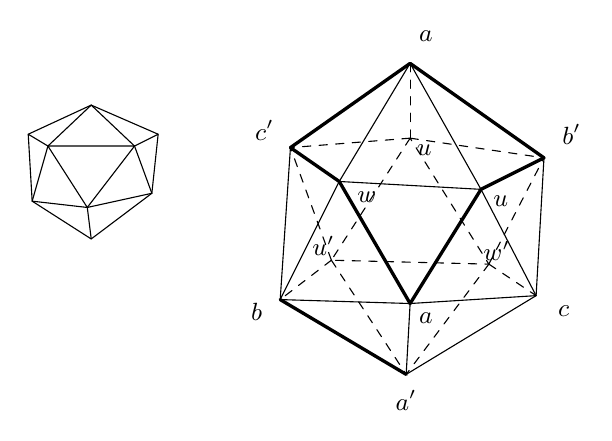
\begin{tikzpicture}[x=1mm,y=1mm,line cap=round,line join=round,font=\scriptsize]
\draw (22,-20.3) -- (30.5,-24) -- (29.7,-31.5) -- (22,-37.3) -- (14.5,-32.5) -- (14,-24) -- (22,-20.3);
\draw (16.5,-25.5) -- (27.5,-25.5) -- (21.5,-33.3) -- (16.5,-25.5);
\draw (16.5,-25.5) -- (14,-24);
\draw (16.5,-25.5) -- (22,-20.3);
\draw (16.5,-25.5) -- (14.5,-32.5);
\draw (27.5,-25.5) -- (22,-20.3);
\draw (27.5,-25.5) -- (30.5,-24);
\draw (27.5,-25.5) -- (29.7,-31.5);
\draw (21.5,-33.3) -- (14.5,-32.5);
\draw (21.5,-33.3) -- (22,-37.3);
\draw (21.5,-33.3) -- (29.7,-31.5);
\draw[very thick] (47.3,-25.7) -- (62.5,-15) -- (79.5,-27);
\draw (79.5,-27) -- (78.5,-44.5) -- (62,-54.5);
\draw[very thick] (62,-54.5) -- (46,-45);
\draw (46,-45) -- (47.3,-25.7);
\draw (53.5,-30) -- (71.5,-31);
\draw[very thick] (71.5,-31) -- (62.5,-45.5) -- (53.5,-30);
\draw[very thick] (53.5,-30) -- (47.3,-25.7);
\draw (53.5,-30) -- (62.5,-15);
\draw (53.5,-30) -- (46,-45);
\draw (71.5,-31) -- (62.5,-15);
\draw[very thick] (71.5,-31) -- (79.5,-27);
\draw (71.5,-31) -- (78.5,-44.5);
\draw (62.5,-45.5) -- (46,-45);
\draw (62.5,-45.5) -- (62,-54.5);
\draw (62.5,-45.5) -- (78.5,-44.5);
\draw[dashed] (62.5,-24.5) -- (52.5,-40) -- (72.5,-40.5) -- (62.5,-24.5);
\draw[dashed] (62.5,-24.5) -- (62.5,-15);
\draw[dashed] (62.5,-24.5) -- (47.3,-25.7);
\draw[dashed] (62.5,-24.5) -- (79.5,-27);
\draw[dashed] (52.5,-40) -- (47.3,-25.7);
\draw[dashed] (52.5,-40) -- (46,-45);
\draw[dashed] (52.5,-40) -- (62,-54.5);
\draw[dashed] (72.5,-40.5) -- (79.5,-27);
\draw[dashed] (72.5,-40.5) -- (78.5,-44.5);
\draw[dashed] (72.5,-40.5) -- (62,-54.5);
\node[inner sep=1pt] at (64.5,-11.5) {\small $a$};
\node[inner sep=1pt] at (83,-24) {\small $b'$};
\node[inner sep=1pt] at (82,-46.5) {\small $c$};
\node[inner sep=1pt] at (62,-57.8) {\small $a'$};
\node[inner sep=1pt] at (43,-46.5) {\small $b$};
\node[inner sep=1pt] at (44,-23.5) {\small $c'$};
\node[inner sep=1pt] at (57,-32) {\small $w$};
\node[inner sep=1pt] at (74,-32.5) {\small $u$};
\node[inner sep=1pt] at (64.5,-47.3) {\small $a$};
\node[inner sep=1pt] at (64.3,-26) {\small $u$};
\node[inner sep=1pt] at (51.5,-38.2) {\small $u'$};
\node[inner sep=1pt] at (73.5,-38.8) {\small $w'$};
\end{tikzpicture}
\end{document}
